\documentclass[10pt,letterpaper,twocolumn]{article}
\usepackage[top=0.75in,bottom=1in,left=0.625in,right=0.625in,columnsep=0.25in]{geometry}
\usepackage{mathptmx}
\usepackage{amsmath}
\usepackage{graphicx}
\usepackage{booktabs,array}
\usepackage{cite}
\usepackage{tikz}
\usetikzlibrary{arrows.meta,positioning}
\usepackage{titlesec}
\usepackage{caption}
\usepackage{enumitem}
\usepackage[hidelinks]{hyperref}

\pagestyle{empty}
\setlength{\parindent}{1em}
\setlength{\parskip}{0pt}
\renewcommand{\baselinestretch}{1.0}
\sloppy

\renewcommand{\thesection}{\Roman{section}}
\renewcommand{\thesubsection}{\Alph{subsection}}
\titleformat{\section}[block]{\centering\scshape\small}{\thesection.}{0.6em}{}
\titleformat{\subsection}[block]{\itshape\small}{\thesubsection.}{0.5em}{}
\titlespacing*{\section}{0pt}{9pt}{4pt}
\titlespacing*{\subsection}{0pt}{6pt}{2pt}

\renewcommand{\thetable}{\Roman{table}}
\captionsetup[figure]{name={Fig.},labelsep=period,font={footnotesize},justification=centering}
\captionsetup[table]{name={TABLE},labelsep=newline,font={footnotesize},textfont=sc,justification=centering,skip=3pt}
\setlist{nosep,leftmargin=1.4em}

\newcommand{\IEEEkeywords}[1]{\par\noindent{\fontsize{9}{10.5}\selectfont\bfseries\itshape Index Terms\,---\,#1\par}}

\begin{document}

\twocolumn[
\begin{center}
{\fontsize{22}{26}\selectfont JalRakshak: A Low-Cost IoT-Based Water Purification and Quality Monitoring System for Rural and Mining-Affected Areas of Jharkhand\par}
\vspace{10pt}
{\fontsize{11}{13}\selectfont Nischal Kumar Singhania (SAP ID 590015167) \hspace{2em} Animesh Giri (SAP ID 590012563)\par}
\vspace{2pt}
{\small\itshape B.Tech Computer Science and Engineering, Third Year\par}
\vspace{3pt}
{\footnotesize Prototype evaluation on simulated data; field validation remains pending\par}
\end{center}
\vspace{6pt}
]

\noindent{\fontsize{9}{10.5}\selectfont\bfseries\itshape Abstract\,---\,JalRakshak is a low-cost water purification and quality-monitoring prototype intended for rural and mining-affected communities in Jharkhand. The proposed treatment train combines sediment filtration, activated carbon, membrane treatment selected after water analysis, and UV disinfection. Its monitoring design tracks pH, turbidity, total dissolved solids (TDS) and temperature on raw and treated lines. The completed software prototype includes a six-view browser dashboard, a FastAPI ingestion service, per-device API-key checks, SQLite persistence, threshold-based alerts, a seeded data generator and model-evaluation scripts. A reproducible simulator generated 504 hourly records for three illustrative units. With a chronological 70/30 split, persistence achieved lower one-hour forecast error than linear regression and random forest for TDS and turbidity. Isolation Forest reached precision 0.796, recall 0.582 and F1-score 0.672 on the held-out synthetic records. A further ten-condition sensitivity sweep examined noise, missing readings and sensor drift. These measurements validate software behaviour only. The ESP32 firmware is an integration template, and no physical sensors, water samples or laboratory tests were available. Thus the 100\% completion reported here applies to the software prototype, not a field-ready purifier or drinking-water certification.\par}

\IEEEkeywords{water quality monitoring, IoT, ESP32, TDS, turbidity, anomaly detection, Isolation Forest, time-series forecasting, rural water supply}

%------------------------------------------------------------
\section{Introduction}
Access to safe drinking water remains a serious problem in parts of rural India. In coal-mining districts of Jharkhand such as Dhanbad, studies of the Jharia coalfield have examined how mining affects the groundwater that nearby villages depend on \cite{panigrahy2015}, and heavy-metal contamination of water and soil has been reported near other Jharkhand coalfields \cite{singh2015}. Households in these areas rarely have laboratory access, so they cannot tell when their water becomes unsafe or when a purifier has stopped working.

Commercial purifiers treat water but usually report little about it, while stand-alone TDS meters report one number without context or history. IoT monitoring systems with pH, turbidity, TDS and temperature sensors have been demonstrated widely \cite{sung2021,salehin2023,marifah2025}, but a system for remote communities has to combine purification, monitoring, understandable alerts and trend analysis, work with limited power and connectivity, and be honest about what its sensors cannot detect.

This work targets that combination. The contributions reported here are:
\begin{itemize}
\item an end-to-end local software architecture with a FastAPI ingestion service, device-key validation, SQLite persistence and a browser dashboard (Section~IV);
\item parameter-specific alert rules that distinguish acceptable and permissible limits without making a potability claim (Section~IV-E);
\item a seeded 504-row synthetic dataset with injected sensor and filter-degradation scenarios (Section~V-A);
\item a chronological forecast/anomaly evaluation and a ten-condition sensitivity sweep (Sections~V-B to V-D); and
\item a runnable dashboard/API package, a device-firmware integration template and explicit hardware/laboratory limitations (Sections~VI and VIII).
\end{itemize}
Section~II reviews related work, Section~III states the problem, Sections~IV and V describe the design and methods, Section~VI reports the prototype and experiment results, and Sections~VII to IX discuss limitations, conclusions and future work.

%------------------------------------------------------------
\section{Background and Related Work}
\subsection{Water Quality in Mining-Affected Regions}
Panigrahy \emph{et al.} analysed 29 groundwater samples from the Jharia coalfield in Dhanbad across seasons and found pH from slightly acidic to slightly alkaline, with water generally suitable for domestic use apart from some exceptions \cite{panigrahy2015}. Singh \emph{et al.} measured metals including Fe, Cu, Zn, Mn, Pb, Cd and Ni in water and soil of the Simlong coalfield in Sahebganj \cite{singh2015}. These studies show that quality varies by place and season and that contaminants of concern include metals, which low-cost physical sensors do not measure. Periodic laboratory testing therefore remains necessary.

\subsection{Standards}
The Bureau of Indian Standards lists IS~10500:2012 (Second Revision) as reviewed in 2023, with four amendments \cite{bis}. The pH acceptable range is 6.5--8.5 with no relaxation; turbidity and TDS have acceptable and permissible limits shown in Table~I. The values are configuration defaults for this prototype and must be checked against the applicable amended standard and local requirements before deployment. The current WHO fourth edition incorporating the first, second and third addenda was issued in 2026 and emphasises risk management and independent surveillance; chemical and microbiological testing remains necessary for a complete assessment \cite{who}.

\subsection{IoT Water Quality Monitoring}
Sung \emph{et al.} built an Arduino-based system measuring turbidity, temperature, pH, conductivity and TDS and sending the data over the internet \cite{sung2021}. Salehin \emph{et al.} describe a low-cost IoT monitoring system for turbidity, TDS, pH and temperature \cite{salehin2023}. Ma'rifah \emph{et al.} describe a rural monitoring and filtration system using pH, TDS and turbidity sensors, a Blynk dashboard, Telegram notifications and field tests in Indonesia \cite{marifah2025}. Our design follows this general sensor set but adds raw-versus-purified comparison, per-stage health tracking, forecasting, anomaly detection and an explicit evaluation protocol.

\subsection{Anomaly Detection and Forecasting}
Anomaly detection methods are surveyed in \cite{chandola2009}. Isolation Forest \cite{liu2008} isolates points with random partitions and needs no labelled anomalies, which suits sensor streams where contamination events are rare. For forecasting we compare a persistence baseline with regression models, including random forests \cite{breiman2001}, using MAE and RMSE \cite{hyndman2006}; implementations come from scikit-learn \cite{sklearn}.

\subsection{Gap}
Existing systems demonstrate sensing and display. We have not found, in the sources reviewed, one that evaluates forecasting, anomaly alerts and robustness together on a purifier-with-monitor prototype; a broader literature review is still required before any claim of novelty is made.

%------------------------------------------------------------
\section{Problem Statement and Research Questions}
\textbf{Problem.} Design a low-cost, portable, energy-efficient unit that purifies contaminated water and continuously reports its quality, with understandable warnings, for communities with limited infrastructure.

\textbf{Research questions.} \textbf{RQ1:} Does a simple ML model forecast purified-water TDS and turbidity with lower error than a persistence baseline? \textbf{RQ2:} Can Isolation Forest flag injected sensor spikes and contamination events with useful precision and recall? \textbf{RQ3:} Can alerts state what changed (for example a turbidity surge or a worn membrane)? \textbf{RQ4:} How do sensor noise, missing readings and drift affect RQ1 and RQ2?

%------------------------------------------------------------
\section{System Design}
\subsection{Architecture}
Fig.~1 shows the implemented local software flow and the future sensor input point. The local software path is operational: the FastAPI service accepts authenticated readings, validates device identity and sensor ranges, stores records and rule-based alerts in SQLite, and serves the dashboard. The seed loader copies the 504-row CSV into the same SQLite database used by the dashboard. The dashboard reads stored series through the API, while the forecasting, anomaly and robustness experiments read the reproducible CSV directly as Python jobs. An ESP32 firmware template is supplied for the future sensor node, but physical probe calibration and live hardware-to-server transmission have not been tested.

\begin{figure}[t]
\centering
\resizebox{\columnwidth}{!}{%
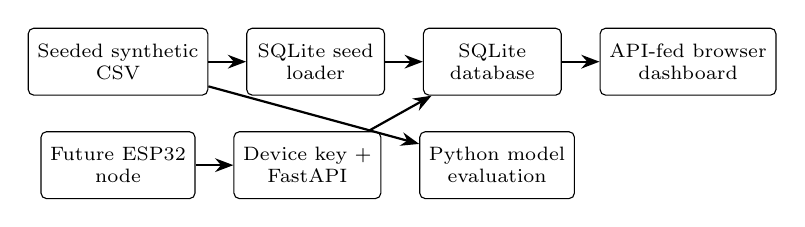
\begin{tikzpicture}[node distance=0.45cm and 0.48cm,
 box/.style={draw,rounded corners=2pt,align=center,minimum height=0.85cm,minimum width=1.75cm,font=\scriptsize},
 arr/.style={-{Stealth},thick}]
 \node[box] (csv) {Seeded synthetic\\CSV};
 \node[box,right=of csv] (seed) {SQLite seed\\loader};
 \node[box,right=of seed] (db) {SQLite\\database};
 \node[box,right=of db] (ui) {API-fed browser\\dashboard};
 \node[box,below=of csv] (esp) {Future ESP32\\node};
 \node[box,right=of esp] (api) {Device key +\\FastAPI};
 \node[box,right=of api] (ml) {Python model\\evaluation};
 \draw[arr] (csv)--(seed); \draw[arr] (seed)--(db); \draw[arr] (db)--(ui);
 \draw[arr] (esp)--(api); \draw[arr] (api)--(db);
 \draw[arr] (csv)--(ml);
\end{tikzpicture}}
\caption{Distinct data paths: the synthetic CSV is seeded directly into SQLite for the dashboard and is also read by Python experiments; a future ESP32 node will submit telemetry through device-key authenticated FastAPI ingestion.}
\end{figure}

\subsection{Purification Train}
The proposed treatment sequence is sediment filtration for suspended particles, activated carbon for selected organics and taste/odour compounds, membrane treatment selected from source-water analysis, and UV disinfection after adequate clarification. Ultrafiltration alone does not remove dissolved salts and cannot be assumed to remove dissolved metals; reverse osmosis or contaminant-specific media may be required depending on laboratory results. The system must also account for reject-water management, membrane fouling, pretreatment and validated UV dose/flow. The dashboard's remaining-life percentages are illustrative maintenance estimates generated by the prototype, not measured filter-life data.

\subsection{Sensing}
The proposed raw-water and treated-water lines each use a pH probe, a turbidity sensor (NTU), a TDS/conductivity probe and a temperature probe. The ESP32 integration template uses two ADS1115 ADC modules and two DS18B20 probes so that both water lines can be read; the exact sensor modules and electrical conditioning must be selected against manufacturer specifications. pH requires buffer calibration, turbidity requires reference standards, TDS requires a conductivity reference and temperature compensation, and temperature probes require comparison to a reference thermometer. The firmware refuses transmission while pH/turbidity calibration coefficients are unset. No physical probe was connected in this study.

\subsection{Data Model}
The implemented SQLite schema contains \emph{devices} (device id, name, district and location), \emph{readings} (device id, UTC timestamp, source, firmware version and JSON raw/purified sensor fields) and \emph{alerts} (device, source reading, parameter, severity, value, message, status and creation time). The API exposes device, reading, dashboard and alert endpoints. Each device has a distinct API key supplied through environment configuration; an ingestion request must match the key to the submitted device id. Duplicate device/timestamp pairs are rejected, sensor ranges are validated and alert status updates persist in the database. A seeded demo loader imports the synthetic dataset directly for quick local setup.

\subsection{Status and Alert Logic}
The overall status uses the worst monitored parameter. pH outside 6.5--8.5 is marked out of range because IS~10500 provides no relaxation. Turbidity above 1 and up to 5 NTU, or TDS above 500 and up to 2000 mg/L, is marked caution; values above those permissible limits are out of range. API alerts are stored with a parameter, value, severity and plain-language check. The prototype status is not a potability decision: these sensors do not measure pathogens or quantify specific dissolved metals.

\begin{table}[t]
\caption{Default Limits Used for Purified Water}
\centering\small
\begin{tabular}{lccc}
\toprule
Parameter & Preferred & Permissible & Unit\\
\midrule
pH & 6.5--8.5 & No relaxation & --\\
Turbidity & 1 & 5 & NTU\\
TDS & 500 & 2000 & mg/L\\
Temperature & \multicolumn{2}{c}{information only} & $^\circ$C\\
\bottomrule
\end{tabular}
\end{table}

%------------------------------------------------------------
\section{Methodology}
\subsection{Simulated Data Generator}
A seeded pseudo-random generator creates 168 hourly records for each of three illustrative units (504 rows total). Raw pH, TDS, turbidity and temperature vary around the unit-specific starting values. Purified TDS is calculated using an assumed removal ratio $\eta_t$, and purified turbidity is estimated as $0.15+0.04\times$ raw turbidity with small noise. The simulator injects a six-hour turbidity surge, gradual membrane degradation, a TDS drift, a stuck pH sensor and a short TDS dropout. The seed is fixed at 42. All removal ratios and event profiles are simulator assumptions, not measured filter performance or observed contamination.

\begin{table}[t]
\caption{Simulated Units}
\centering\footnotesize
\begin{tabular}{@{}llrrr>{\raggedright\arraybackslash}p{1.2in}@{}}
\toprule
ID & District & pH & NTU & TDS & Scenario\\
\midrule
JW-01 & Dhanbad & 7.4 & 8 & 780 & 6-h turbidity surge (+11 to +66 NTU)\\
JW-02 & W. Singhbhum & 7.9 & 4 & 1350 & high-TDS source, no event\\
JW-03 & Ramgarh & 7.1 & 3 & 900 & membrane wear: $\eta$ falls 0.90$\to$0.39 over 44 h\\
\bottomrule
\end{tabular}
\end{table}

\subsection{Forecasting}
The target is purified-water TDS and turbidity one hour ahead. Features include lagged raw and purified sensor values, six-hour rolling means and standard deviations, and cyclic hour-of-day terms. The compared models are a persistence baseline $\hat y_{t+1}=y_t$, linear regression and a random forest regressor. For each device, the first 70\% of the hourly sequence is used for training and the final 30\% is held out for testing. Feature construction uses past and current readings only; no test labels or future readings are used for fitting. Errors are
\begin{equation}
\mathrm{MAE}=\tfrac1n\sum_i|y_i-\hat y_i|,\quad
\mathrm{RMSE}=\sqrt{\tfrac1n\sum_i(y_i-\hat y_i)^2}.
\end{equation}

\subsection{Anomaly Detection}
An Isolation Forest scores a sample $x$ as $s(x,n)=2^{-E[h(x)]/c(n)}$, where $h(x)$ is its path length in random trees and $c(n)$ normalises by sample size \cite{liu2008}. Inputs include the four purified-water parameters, raw TDS and turbidity, a TDS ratio, sensor differences and a dropout indicator. Ground truth comes from the injected events (turbidity surge, membrane degradation, stuck pH sensor, TDS drift and reading dropout). Isolation Forest is fitted on the first 70\% of each unit. Its anomaly threshold is set at the fifth percentile of training scores only; precision, recall and $F_1$ are then calculated on the held-out rows. Because injected events are easier than real ones, this evaluation shows workflow behaviour, not field accuracy. A flagged anomaly is a warning to investigate, not proof of contamination; a faulty sensor produces similar patterns.

\subsection{Robustness}
A deterministic sensitivity sweep was added after the main experiment. It evaluates three Gaussian-noise levels (2%, 5% and 10% of each channel's dataset standard deviation), three random missing-reading rates (5%, 10% and 20% per device) and three linear purified-TDS drift magnitudes (1%, 3% and 5% of the device's baseline TDS standard deviation), in addition to the unmodified baseline. The same chronological split and training-only anomaly threshold are re-applied in each scenario. At 10% noise, persistence TDS MAE rises from 9.34 to 13.10 mg/L and anomaly F1 is 0.516. At 20% missingness, persistence TDS MAE is 9.81 mg/L on 117 available targets and anomaly F1 falls to 0.417. At 5% drift, anomaly F1 is 0.774; this non-monotonic change reflects the way synthetic event patterns interact with the detector and should not be interpreted as drift improving a real system. These are controlled simulator stress tests, not field robustness results.

%------------------------------------------------------------
\section{Prototype Status and Demonstration}
\subsection{Implemented Components}
The dashboard contains six views: overview, analytics, devices, alerts, forecast/anomaly results and project progress. It supports parameter and time-window selection, raw-versus-purified charts, device selection and alert acknowledgement/resolution. When served by FastAPI, it loads stored readings from the API; it retains a clearly labelled embedded simulation preview when opened as a standalone file. The API provides authenticated ingestion, schema validation, duplicate protection, SQLite persistence and persisted alert updates. The Python package regenerates the dataset, forecast metrics, anomaly scores and sensitivity sweep. Seventeen automated tests cover API authentication, device identity, range checks, timezone requirements, duplicate rejection, persistence, alert rules, dashboard retrieval, data reproducibility and robustness-scenario integrity.

All twelve scoped software deliverables are complete in this release, so the dashboard reports 100\% software-prototype implementation. This score does not include physical deployment. Three external tasks remain outside that denominator: sensor wiring and calibration, purification/laboratory validation, and a permitted field trial. The ESP32 source is an integration template and has not been compiled against the final sensor hardware or tested on a board.

\subsection{Synthetic Data Summary}
Table~III reports the mean values produced by the current seed-42 generator. The raw-to-purified differences are determined by the assumed removal ratios in the simulator. They are not a measured filtration efficiency. The JW-01 surge produces several turbidity-limit exceedances, while the JW-03 membrane scenario raises simulated purified TDS above the preferred 500 mg/L line.

\begin{table}[t]
\caption{Seed-42 Simulated Seven-Day Mean Values}
\centering\footnotesize
\begin{tabular}{@{}lrrrr@{}}
\toprule
 & \multicolumn{2}{c}{TDS (mg/L)} & \multicolumn{2}{c}{Turbidity (NTU)}\\
\cmidrule(lr){2-3}\cmidrule(lr){4-5}
Unit & Raw & Purified & Raw & Purified\\
\midrule
JW-01 & 783.2 & 78.2 & 9.18 & 0.52\\
JW-02 & 1344.5 & 113.7 & 4.01 & 0.31\\
JW-03 & 898.5 & 149.6 & 2.99 & 0.27\\
\bottomrule
\end{tabular}
\end{table}

\begin{figure}[t]
\centering
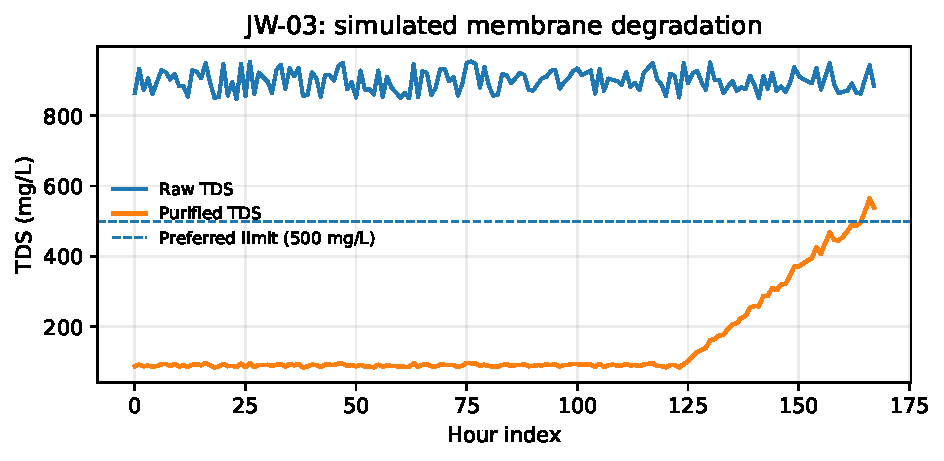
\includegraphics[width=\columnwidth]{jw03_tds_series.pdf}
\caption{Purified TDS rises in the JW-03 synthetic membrane-degradation scenario. Both the raw and purified traces are simulated.}
\end{figure}

%------------------------------------------------------------
\section{Evaluation Results on the Simulated Test Set}
Table~IV gives one-hour-ahead forecasting errors on the held-out period: 150 observed TDS targets (three missing TDS readings are excluded) and 153 turbidity targets. Persistence achieved the lowest error for both parameters. On this generated series, the regressors did not improve on simply carrying the latest reading forward. This is a useful negative result: adding model complexity did not improve the short-horizon forecast under the current assumptions.

\begin{table}[t]
\caption{One-Hour-Ahead Forecasting Results (Simulated Test Set)}
\centering\footnotesize
\begin{tabular}{@{}lrrrr@{}}
\toprule
 & \multicolumn{2}{c}{TDS} & \multicolumn{2}{c}{Turbidity}\\
\cmidrule(lr){2-3}\cmidrule(lr){4-5}
Model & MAE & RMSE & MAE & RMSE\\
\midrule
Persistence & 9.34 & 20.39 & 0.080 & 0.247\\
Linear regression & 79.02 & 147.31 & 0.278 & 0.516\\
Random forest & 74.05 & 143.94 & 0.093 & 0.332\\
\bottomrule
\end{tabular}
\end{table}

For anomaly detection, Isolation Forest reached precision 0.796, recall 0.582 and $F_1=0.672$ across 153 held-out rows, of which 67 carried injected event labels. Per-device $F_1$ values were 0.444 (JW-01), 0.643 (JW-02) and 0.743 (JW-03). The threshold was selected using training scores only. The detector missed some injected events and should not be treated as a contamination classifier.

\begin{table}[t]
\caption{Selected Simulator Sensitivity Results}
\centering\footnotesize
\begin{tabular}{@{}lrrr@{}}
\toprule
Scenario & TDS persistence MAE & Anomaly F1 & TDS targets\\
\midrule
Baseline & 9.34 & 0.672 & 150\\
10\% sensor noise & 13.10 & 0.516 & 150\\
5\% missing readings & 9.49 & 0.673 & 147\\
10\% missing readings & 10.17 & 0.552 & 133\\
20\% missing readings & 9.81 & 0.417 & 117\\
5\% linear drift & 9.35 & 0.774 & 150\\
\bottomrule
\end{tabular}
\end{table}

These numbers are reproducible checks on synthetic data, not an estimate of performance in Jharkhand villages. Because the same generator determines both the signals and event labels, the test checks implementation and time-split discipline but cannot establish external validity. The sensitivity sweep further shows that missingness and noise can alter both forecast errors and anomaly recall, so thresholds and models must be re-evaluated using calibrated field probes and separately labelled laboratory/site data.

%------------------------------------------------------------
\section{Discussion and Limitations}
\textbf{Sensor limits.} pH, turbidity, TDS and temperature probes do not directly detect pathogens or heavy metals such as arsenic, lead, iron and fluoride \cite{singh2015}. UV disinfection is effective only when correctly selected, maintained and operated; metals still require appropriate treatment and laboratory analysis. The dashboard reports only monitored parameters and does not certify potability. \textbf{Synthetic evidence.} All model scores and water-quality values come from a generator whose assumptions are known. They do not describe field conditions, probe errors or actual filter performance. \textbf{Calibration.} Low-cost probes need reference calibration and drift checks; TDS readings depend on temperature. \textbf{Standards.} Limits must be checked against the latest amended IS~10500 and local guidance before deployment. \textbf{Generalisation.} Three simulated units and one week of data cannot represent other sites, seasons or mine-water chemistry \cite{panigrahy2015}.

%------------------------------------------------------------
\section{Conclusion and Future Work}
This release delivers a complete local software prototype: six dashboard views, a FastAPI service, device-key authentication, SQLite persistence, alert workflows, a reproducible 504-row data generator, forecasting and anomaly experiments, a ten-condition sensitivity sweep, automated tests and an ESP32 integration template. Persistence remained the strongest one-hour forecast baseline on the generated stream. Isolation Forest detected some injected events, but its recall changed under noise and missingness. The results describe the simulator only. The next stage is physical: select sensor models, design safe analogue conditioning and enclosure, calibrate each probe, build the treatment train from source-water laboratory results, test treated samples against accredited laboratory analysis and complete supervised field trials. The software prototype is complete; physical treatment performance and drinking-water safety are not established.

%------------------------------------------------------------
\section{Code and Data Availability}
The repository contains the source code, seeded synthetic CSV, FastAPI/SQLite backend, 17 automated tests, ESP32 firmware integration template, forecast and anomaly scripts, robustness sweep, result tables, figures and the interactive dashboard source. Running \texttt{./run\_all.sh} recreates the 504-row dataset, evaluation outputs, sensitivity results, seeds the local demo database and runs the test suite. The dashboard is served at \texttt{http://127.0.0.1:8000/} after starting the API. No field measurements, household records or laboratory data were collected. The public GitHub URL will be added after the student publishes the individual repository; until then, the submitted ZIP is the complete source and data archive.

\footnotesize
\setlength{\itemsep}{0pt}
\setlength{\parskip}{0pt}
\begin{thebibliography}{99}
\bibitem{panigrahy2015} B. P. Panigrahy, P. K. Singh, A. K. Tiwari, and B. Kumar, ``Variation in groundwater quality with seasonal fluctuation in Jharia coal mine region, Jharkhand, India,'' \emph{Curr. World Environ.}, vol. 10, no. 1, pp. 171--178, 2015.
\bibitem{singh2015} R. B. P. Singh, A. Singh, \emph{et al.}, ``Surface mining and heavy metal pollution of water and soil: A case study in Simlong coalfield in Sahebganj district, Jharkhand,'' \emph{IJANS}, vol. 4, no. 1, pp. 17--24, Jan. 2015.
\bibitem{sung2021} W.-T. Sung, F. N. Fadillah, and S.-J. Hsiao, ``IoT-based water quality monitoring,'' \emph{Sens. Mater.}, vol. 33, no. 8, 2021.
\bibitem{salehin2023} S. Salehin, T. A. Meem, A. J. Islam, and N. Al Islam, ``Design and development of a low-cost IoT-based water quality monitoring system,'' Springer, Singapore, 2023.
\bibitem{marifah2025} P. N. Ma'rifah, P. N. Magfirah, E. K. Rahayu, M. Shauqi, I. R. Sukman R. T., and S. Rifandi, ``Smart digital measurement system for rural water quality monitoring using IoT,'' \emph{Jurnal Teknik Elektro dan Komputer TRIAC}, vol. 12, no. 2, 2025, doi: 10.21107/triac.v12i2.32139.
\bibitem{bis} Bureau of Indian Standards, \emph{IS 10500:2012, Drinking Water -- Specification (Second Revision)}, reviewed 2023; Amendments 1--4 (2015, 2018, 2020 and 2021).
\bibitem{who} World Health Organization, \emph{Guidelines for Drinking-water Quality}, 4th ed., incorporating the first, second and third addenda. Geneva, Switzerland, 2026. ISBN 978-92-4-012122-5. \url{https://www.who.int/publications/i/item/9789240121225}.
\bibitem{liu2008} F. T. Liu, K. M. Ting, and Z.-H. Zhou, ``Isolation forest,'' in \emph{Proc. 8th IEEE Int. Conf. Data Mining (ICDM)}, Pisa, Italy, 2008, pp. 413--422.
\bibitem{chandola2009} V. Chandola, A. Banerjee, and V. Kumar, ``Anomaly detection: A survey,'' \emph{ACM Comput. Surv.}, vol. 41, no. 3, Art. 15, 2009.
\bibitem{breiman2001} L. Breiman, ``Random forests,'' \emph{Mach. Learn.}, vol. 45, no. 1, pp. 5--32, 2001.
\bibitem{hyndman2006} R. J. Hyndman and A. B. Koehler, ``Another look at measures of forecast accuracy,'' \emph{Int. J. Forecasting}, vol. 22, no. 4, pp. 679--688, 2006.
\bibitem{sklearn} F. Pedregosa \emph{et al.}, ``Scikit-learn: Machine learning in Python,'' \emph{J. Mach. Learn. Res.}, vol. 12, pp. 2825--2830, 2011.
\bibitem{esp32} Espressif Systems, \emph{ESP32 Series Datasheet}, Version 5.3, consulted 2026, \url{https://www.espressif.com/sites/default/files/documentation/esp32_datasheet_en.pdf}.
\bibitem{fastapi} FastAPI, ``FastAPI documentation,'' \url{https://fastapi.tiangolo.com/}.
\bibitem{sqlite} SQLite Project, ``SQLite documentation,'' \url{https://www.sqlite.org/docs.html}.
\end{thebibliography}

\end{document}
